% !TEX root = ../../../Masterthesis.tex

\section{London Falling}
This cue starts at approximately 0:16:34 right after Kirk's reprimand. A piano plays an arpeggiated \bflatm,(figure \ref{ST12_london_falling_motif_1}) while a solo oboe plays a simple theme: \textbf{theme B}. We see a birds eye view of London. The strings join the arpeggio, steadily intensifying when the main antagonist, Kahn, is using a medical device to extract his own blood into a vial. He places the tube in a container, along with a silver ring and all the while the music crescendos over the same \bflatm; all that changes is the thickness of the orchestration and the dynamic. 
\begin{marginfigure}
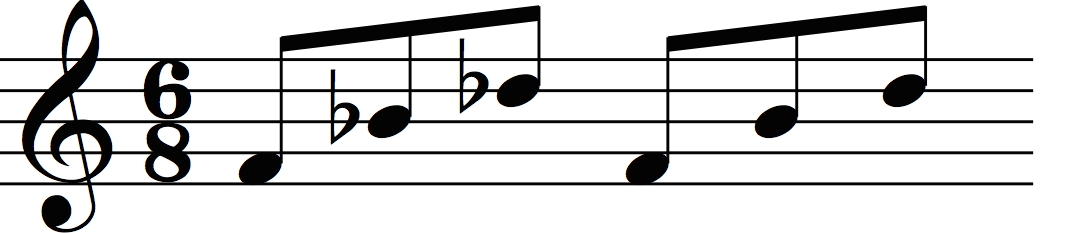
\includegraphics[width=\linewidth]{ST12_london_falling_motif_1}
	\caption{London Falling Motif 1}
	\label{ST12_london_falling_motif_1}
\end{marginfigure}

With \textit{subito piano}, the strings play very lightly in the top register, supporting the solo piano playing \textbf{theme A}. We cut to a living room filled with medical equipment. A mother sleeps on the couch and her child is sleeping in what appears to be a hospital bed while the father enters, carrying the container prepared by Kahn. The man locates the vial and places it into a device that extracts the blood and feeds it to the intravenous apparatus. When this happens, the music shifts slightly; the melody is played an octave higher and the strings enter with an arpeggiated ostinato (figure \ref{ST12_london_falling_motif_2}). A screen showing the girl's vital signs starts blinking and beeping, indicating a positive rise in vital signs. The sad solo piano returns and the pace seems to slow down. The man leans over the sick bed and kisses the girl on the for head, clearly relieved though something still torments him. 

\begin{marginfigure}
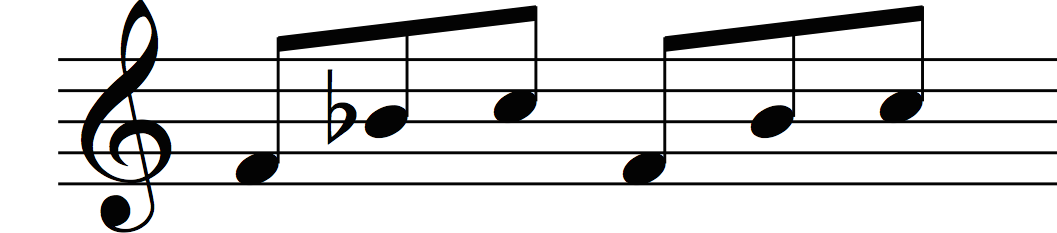
\includegraphics[width=\linewidth]{ST12_london_falling_motif_2}
	\caption{London Falling Motif 2}
	\label{ST12_london_falling_motif_2}
\end{marginfigure}

The scene cuts to the busy streets of London. Motif 2 and 3 (figure \ref{ST12_london_falling_motif_3}) plays simultaneously, creating a driving, ominous tension. The sad piano theme, \textbf{theme A}, now played by flute and oboe, plays on top of the driving pattern. The father, in uniform, walks down the streets and sees Kahn on the opposite side of the street. The music intensifies with long held chords, \textbf{theme B}, and percussion when we see Kahn. The music de-densifies and a new, slightly chromatic and rhythmically unstable theme, \textbf{theme C}, played by oboe, enters as the father passes the security check and enters the elevator.

\begin{marginfigure}
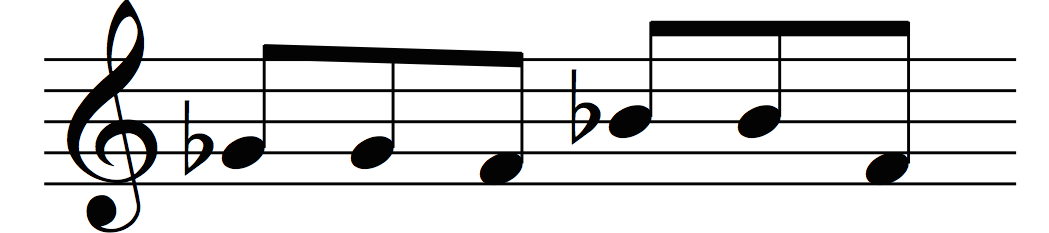
\includegraphics[width=\linewidth]{ST12_london_falling_motif_3}
	\caption{London Falling Motif 3}
	\label{ST12_london_falling_motif_3}
\end{marginfigure}

When we enter the underground research facility, Motif 3 is reinforced by the low strings and percussion as the tension builds. We see the father holding what appears to be a glass of water as he approaches his desk. Hi sits down and activates his workstation. We get a close-up of the father with tears in his eyes. On the computer we see:

\begin{figure}[h!]
\center
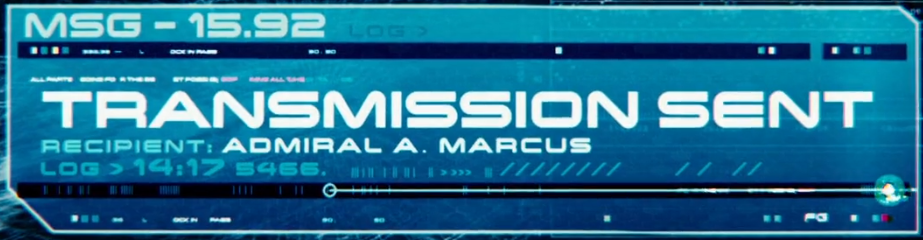
\includegraphics[width=0.7\linewidth]{ST12_transmission_sent}
	\caption{ST12: Transmission Sent}
	\label{ST12_transmission_sent}
	\setfloatalignment{b}
\end{figure}

\noindent We get another close-up, The father, with tears streaming down his face, takes off his silver ring--the ring prepared by Kahn--and drops it into a glass of water. A violent reaction occurs and the entire facility blows up in a high energy explosion.

\begin{figure}
\center
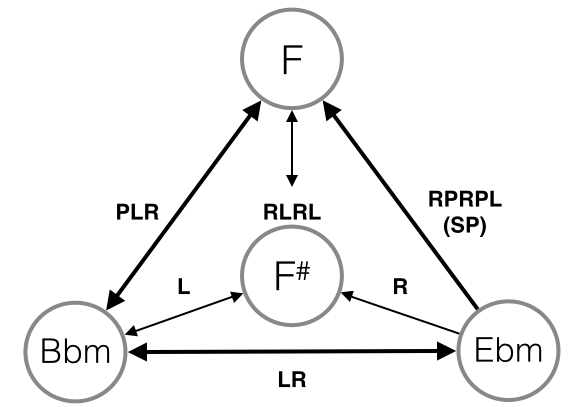
\includegraphics[width=0.7\linewidth]{ST12_london_falling}
	\caption{ST 12: London Falling}
	\label{ST12_london_falling}
	\setfloatalignment{b}
\end{figure}

Giacchino is very economic in his choice of harmony. The tonal center is \bflatm, but the chords used have their axiom centered around \fiss, as closely as possible to the circle of fifths and its minor relatives (figure \ref{ST12_london_falling}). The only exception is F, which is the major dominant in relation to \bflatm. But transformationally, we can see and hear that it feels quite far away tonally. 

%-----------------------------------------------------------------------------
% PDF
%-----------------------------------------------------------------------------
\clearpage
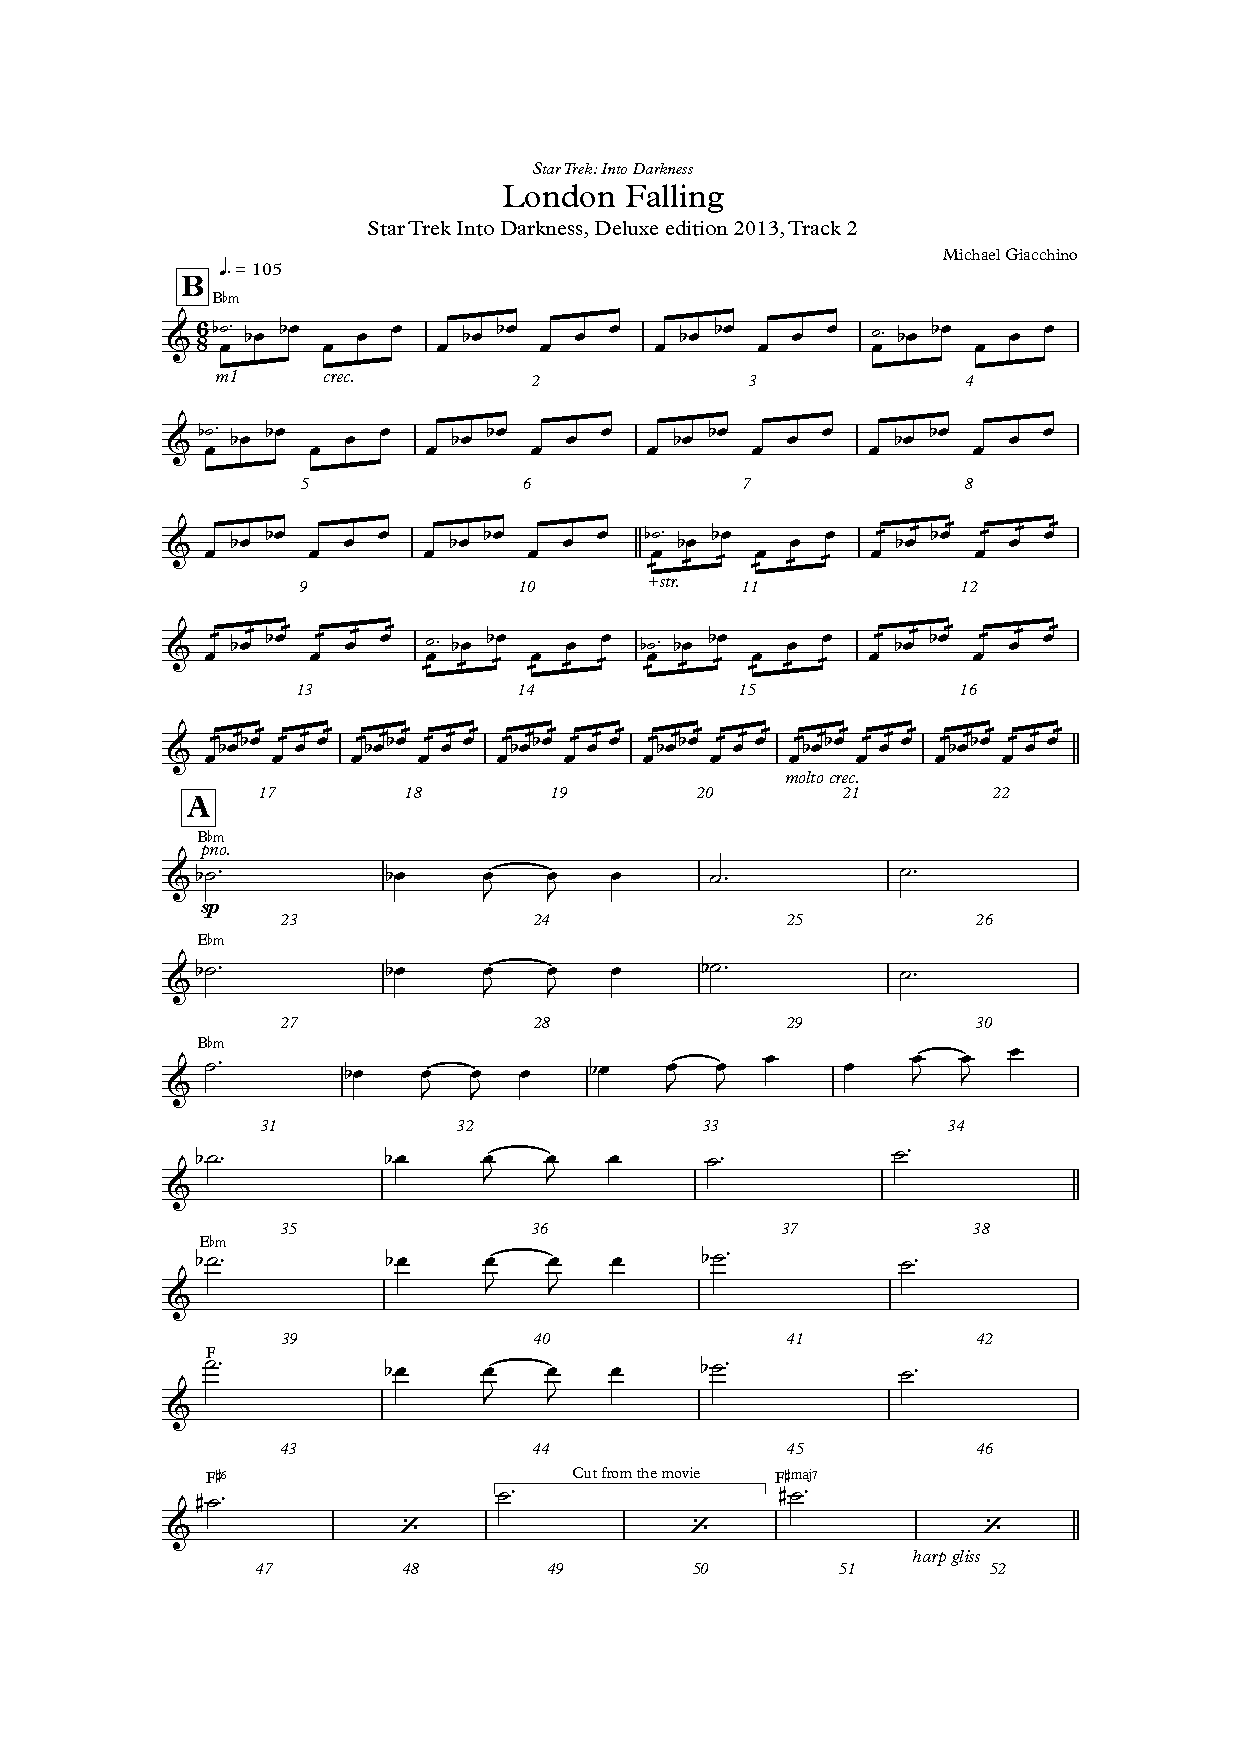
\includepdf[pages=-,pagecommand=\thispagestyle{fancy}]{pdf/st12/ST12_London_Falling.pdf}

% Reviewed